% !Mode:: "TeX:UTF-8"
% \textbf{计算专题------取值说理,与方程结合}

\begin{defproblem}{T16-A02-01}%
\begin{onlyproblem}%
先化简,再求值:$\left(\dfrac{a-2}{a^2+2a}-\dfrac{a-1}{a^2+4a+4}\right)\div \dfrac{a-4}{a+2}$,其中$a$满足$a^{2}+2a-1=0$.
\end{onlyproblem}%
\begin{onlysolution}%
\begin{center}
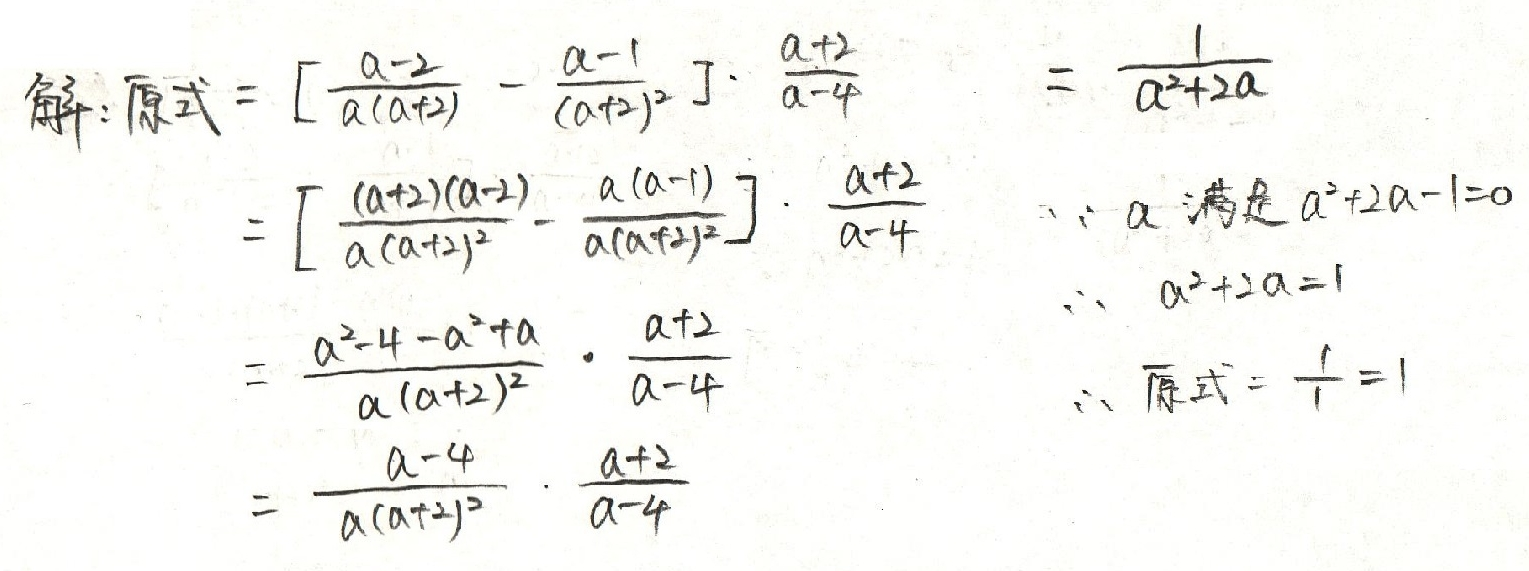
\includegraphics[width=.69\columnwidth]{T16-A02-01.jpg}
\end{center}
\end{onlysolution}%
\end{defproblem}


\begin{defproblem}{T16-A02-02}%
\begin{onlyproblem}%
先化简,再求值$\left(\dfrac{1}{a-b}-\dfrac{b}{a^2-b^2}\right)\div \dfrac{a^2-ab}{a^2-2ab+b^2}$,其中$a$,$b$满足$a+b-\dfrac{1}{2}=0$.
\end{onlyproblem}%
\begin{onlysolution}%
% \begin{center}
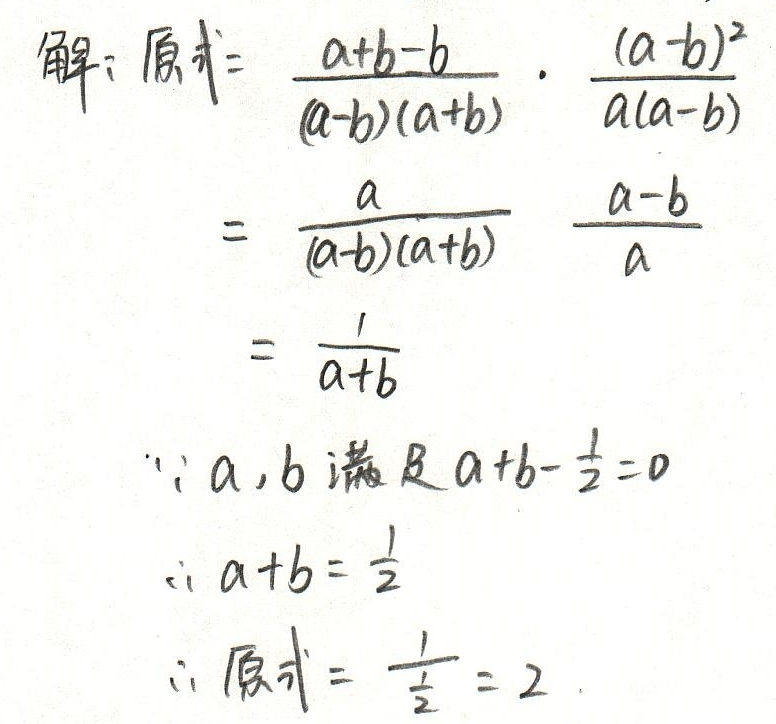
\includegraphics[scale=0.9]{T16-A02-02.jpg}
% \end{center}
\end{onlysolution}%
\end{defproblem}


\begin{defproblem}{T16-A02-03}%
\begin{onlyproblem}%
先化简,再求值:$\dfrac{3m}{3-m}-\left(m+2-\dfrac{5}{m-2}\right)\div \dfrac{9-6m+m^2}{2m-m^2}$,其中$m$是方程$x^{2}=6-2x$的解.
\end{onlyproblem}%
\begin{onlysolution}%
\begin{center}
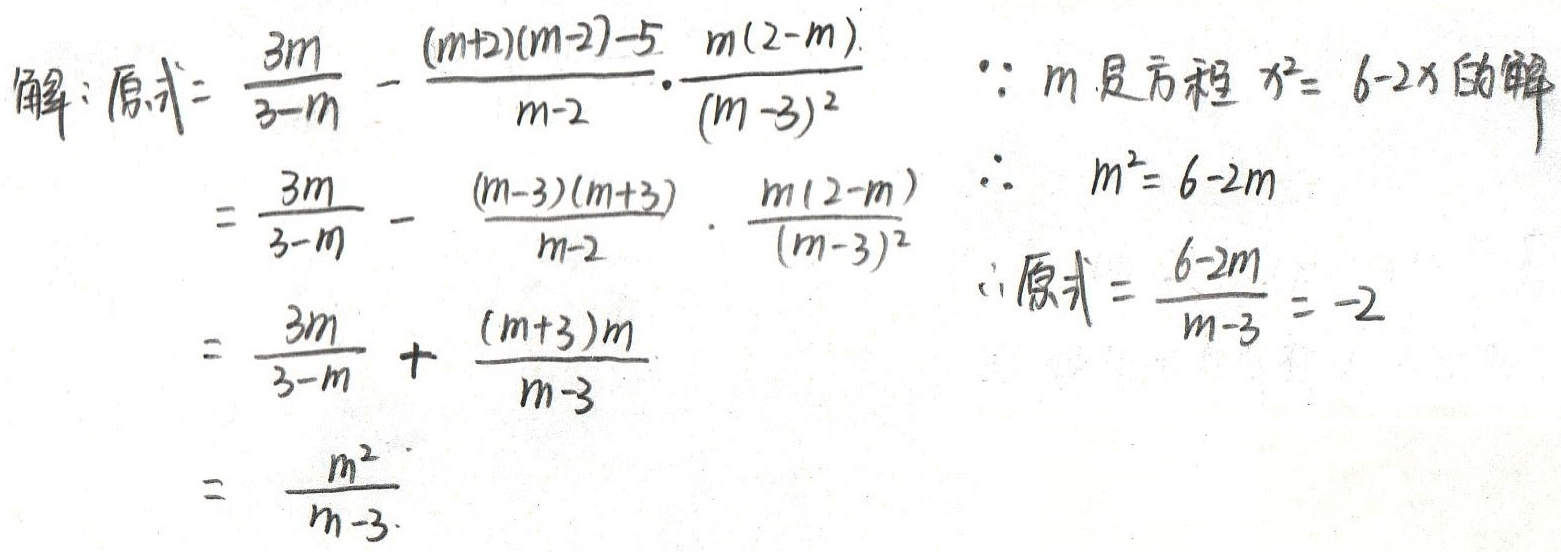
\includegraphics[scale=0.9]{T16-A02-03.jpg}
\end{center}
\end{onlysolution}%
\end{defproblem}


\begin{defproblem}{T16-A02-04}%
\begin{onlyproblem}%
有这样一道题``求$\dfrac{a^2+a}{a^2-1}-\dfrac{a+1}{a^2+2a+1}\div \dfrac{a-1}{a+1}$的值,其中$a=2017$``小马虎''不小心把$a=2 017$错抄成$a=2 007$,但他的计算结果却是正确的,请说明原因.
\end{onlyproblem}%
\begin{onlysolution}%
\begin{center}
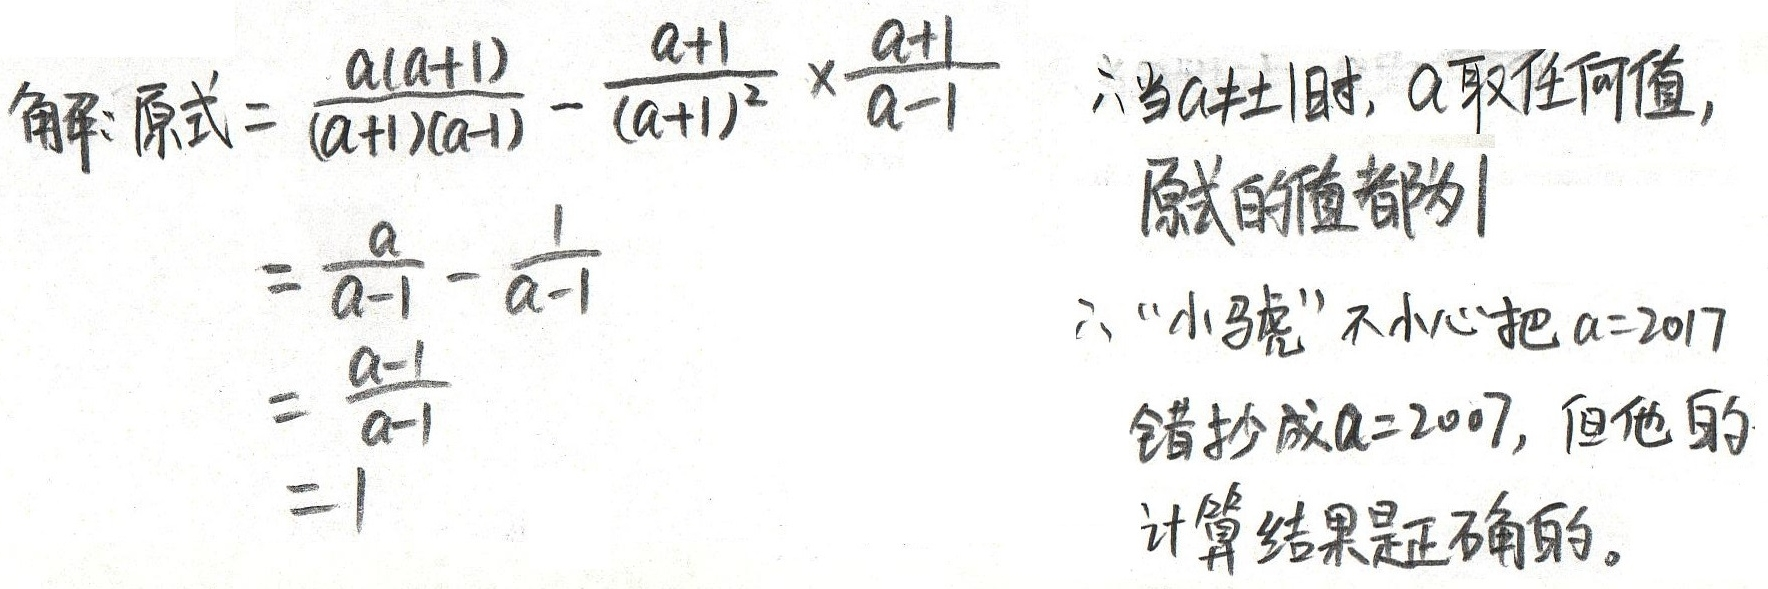
\includegraphics[width=.69\columnwidth]{T16-A02-04.jpg}
\end{center}
\end{onlysolution}%
\end{defproblem}


\begin{defproblem}{T16-A02-05}%
\begin{onlyproblem}%
已知关于$x$的一元二次方程$(a-6)x^{2}-8x+17=0$有实数根.

(1)求$a$的最大整数值.

(2)当$a$取最大整数值时,①求出该方程的根;②求$-2 x^{2}-\dfrac{32x+4}{x^{2}+8x-15}$的值.
\end{onlyproblem}%
\begin{onlysolution}%
\begin{center}
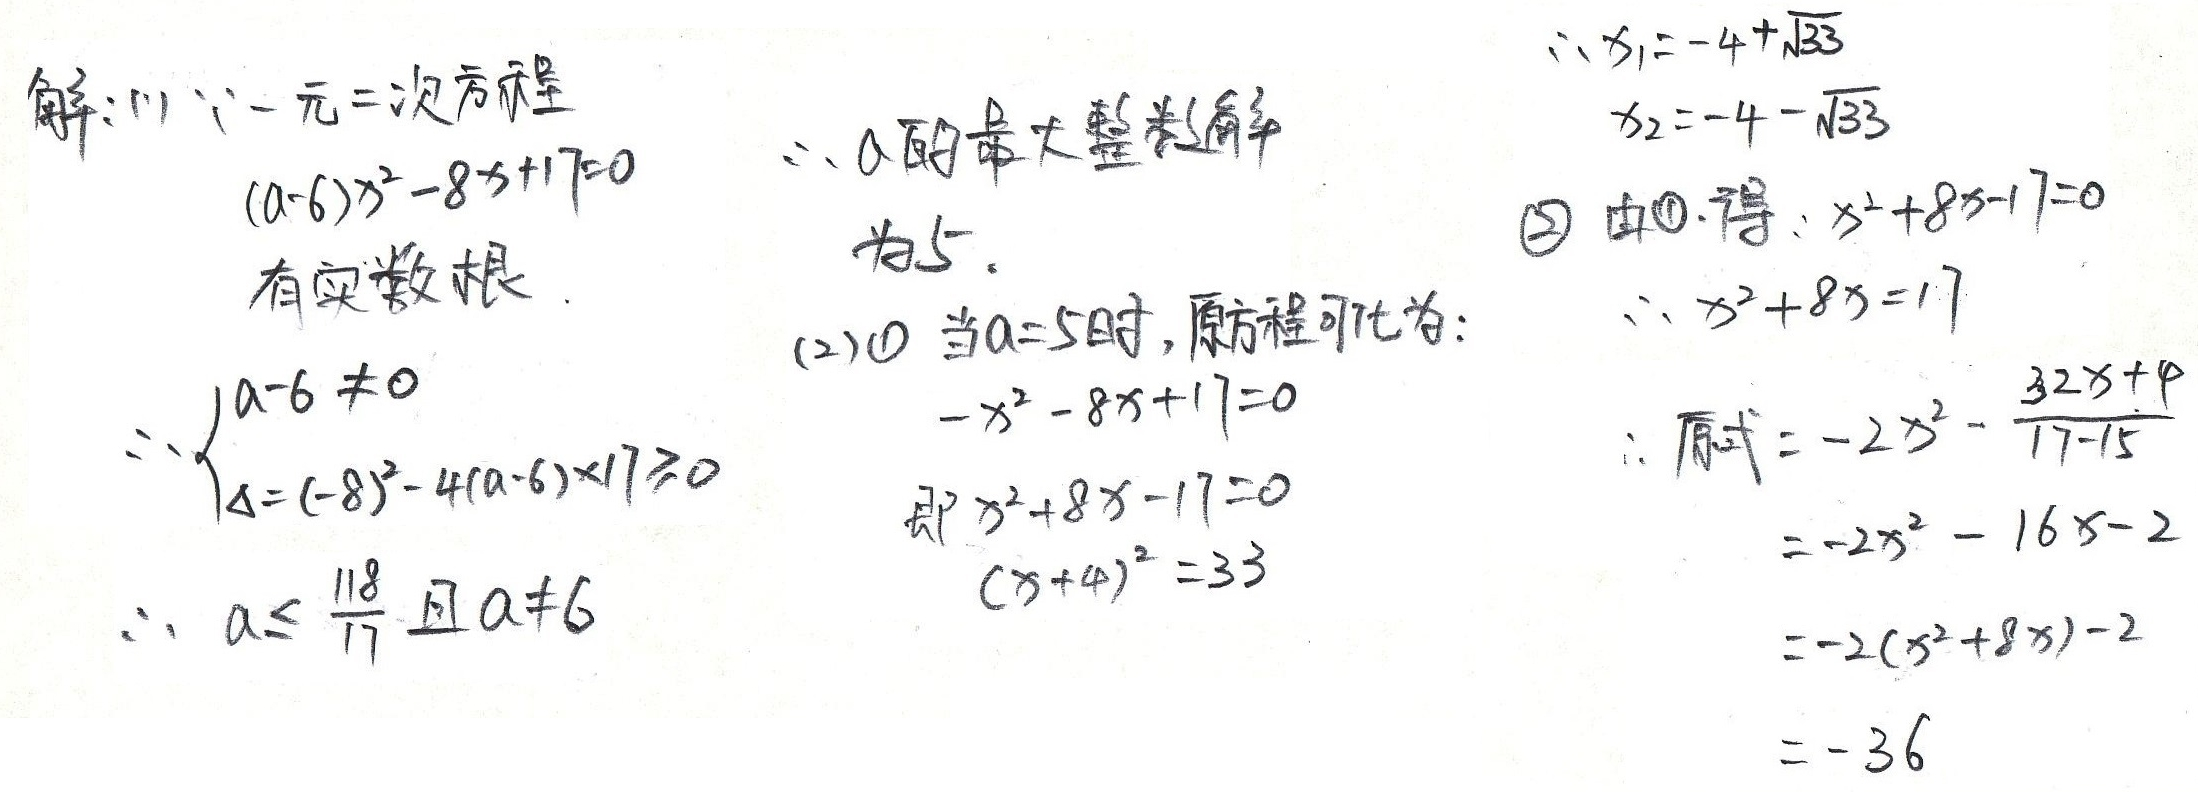
\includegraphics[width=.69\columnwidth]{T16-A02-05.jpg}
\end{center}
\end{onlysolution}%
\end{defproblem}


\begin{defproblem}{T16-A02-06}%
\begin{onlyproblem}%
先化简,再求值:$\dfrac{a}{a+1}\div \left(a-1-\dfrac{2a-1}{a+1}\right)$,并从$-1$,0,1,2四个数中,选一个合适的数代入求值.

\end{onlyproblem}%
\begin{onlysolution}%
\begin{center}
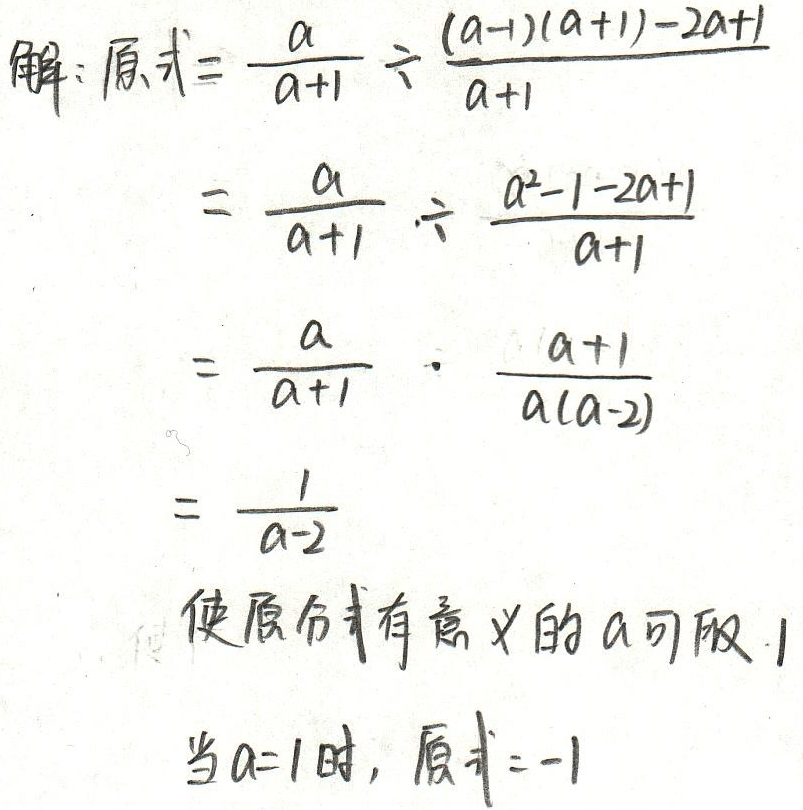
\includegraphics[scale=0.9]{T16-A02-06.jpg}
\end{center}
\end{onlysolution}%
\end{defproblem}

